\begin{appendix}
\chapter{Anexo: Potencial gravitacional de un disco delgado}\label{AnexoA}
El potencial de un disco delgado en la región exterior del mismo, con altura mucho menor que el radio del disco, y simetría axial, se realiza separación de variables.

Expresando la \textbf{ecuación de Laplace} en coordenadas cilíndricas $(R, \phi, z)$ para este sistema con simetría axial y simetría respecto el plano $z=0$, $\Phi = \Phi(R, z) = \Phi(R, -z)$:

\begin{equation}
\label{laplace_eq_disk}
\frac{1}{R} \frac{\partial }{\partial R}  \left ( R \frac{\partial \Phi }{\partial R}  \right ) + \frac{\partial^2 \Phi }{\partial z^2}  = 0,
\end{equation}

donde el potencial es

$$ \Phi(R,z) = J(R) Z(z). $$

Se tiene que la ecuación (\ref{laplace_eq_disk}) se puede escribir en términos de las funciones radial $J(R)$ y de altura $Z(z)$:

\begin{eqnarray}
   Z(z) \frac{1}{R}  \frac{d}{R} \left( R \frac{d J(R)}{R} \right) + J(R) \frac{d^2}{d z^2} Z(z) &=& 0, \\
    \frac{1}{JR} \frac{d}{R}  \left( R \frac{d J(R)}{R} \right) = -\frac{1}{Z}  \frac{d^2}{d R^2} Z(z) &=& -k^2.  \\
\end{eqnarray}

Entonces  la ecuación que depende de $z$ , tiene solución:
$$  \frac{d^2}{d z^2} Z(z)  -k^2 Z(z) = 0    \hspace{1cm}, \hspace{1cm} Z=A e^{kz} + B e^{-kz}, $$

Esta ecuación diferencial para $Z(z)$ en el disco delgado tiene condiciones de frontera $\Phi(R, \infty), \Phi(R, -\infty) \rightarrow 0$, entonces finalmente la solución para la altura es:

\begin{equation}
Z(z) = A e^{-k|z|}.
\end{equation}


La ecuación radial es la definición de la función de Bessel:

\begin{equation}
\label{diff_eq_R}
 \frac{1}{R} \frac{d}{R}  \left( R \frac{d J(R)}{R} \right) + k^2 J(R) = 0.
\end{equation}

La forma general de la ecuación diferencial con soluciones dadas por las funciones de Bessel es:

 $$ \frac{1}{s} \frac{d}{ds}  \left( s \frac{d y}{ds} \right) + \left( k^2 - \frac{\nu^2}{s^2} \right) = 0,  $$

que tiene soluciones $J_{\nu}(ks)$ (primer tipo), $Y_{\nu}(ks)$ (segundo tipo), una familia de funciones de Bessel caracterizadas por el índice $\nu$. La función (\ref{diff_eq_R}) tiene soluciones dadas por la superposición de funciones modificadas de Bessel $J_0(kR), Y_0(kR)$, esto es $\nu = 0$.\\

\subsubsection{Transformada de Hankel}

Para encontrar la solución a la ecuación (\ref{diff_eq_R}) para $J(R)$, se hace uso de la transformada de Hankel. Dada una función $g(r)$, su transformada es:

\begin{equation}
\label{Hankel}
   g'(k) = \int_0^{\infty} g(r) J_{\nu}(kr) r dr,
\end{equation}
y la transformada inversa es

\begin{equation}
\label{inverse_Hankel}
   g(r) = \int_0^{\infty} g'(r) J_{\nu}(kr) k dk.
\end{equation}

Ahora se expresa el potencial en términos de $k$ y así el potencial total es la suma de todos los $\Phi_k$. Los potenciales son la superposición de la solución para $Z(z)$ y para $J_0(kR)$. Podemos generalizar la forma de la solución analizando sólo para $k>0$:

$$ \Phi_k(R,z) = Ce^{-kz} J_0(kR)  \hspace{1cm}, \hspace{1cm} z>0, $$
$$ \Phi_k(R,z) = Ce^{kz} J_0(kR)  \hspace{1cm}, \hspace{1cm} z<0. $$

Entonces la solución para el potencial total está dado por la superposición de estos potenciales $\Phi_k(R,z)$ pesados por una función $f(k)$ que relaciona los factores de escala constantes $C$. Entonces el propósito es encontrar la función de peso para la distribución de masa. En las regiones cercana al plano ecuatorial  del disco $z \rightarrow 0$ y fuera del disco se considera la ecuación de Laplace, y se observa que $\Phi_k$ es continuo cerca al plano, pero $\nabla \Phi_k$ no lo es, dado que depende de $|z|$. Por lo tanto $\nabla^2 \Phi_k = 0$ excepto en $z=0$.\\

Se considera la condición de frontera $\Phi_k \rightarrow 0$ para $R,z \rightarrow \infty$.\\

Para encontrar la distribución de masa volumétrica y por lo tanto la distribución superficial, se usa el Teorema de Gauss para el potencial en una superficie gaussiana cerca al plano $z=0$. Por la ecuación de Poisson:

\begin{equation}
\label{gauss_therorem}
\int_V 4\pi G\rho dV = \int_V \nabla^2\Phi dV = \int_V \nabla \cdot ( \nabla \Phi)  dV = \int_{\Sigma} \nabla \Phi \cdot \textbf{n} d^2 \textbf{S}.
\end{equation}

La altura del disco se hace tender a cero y como se muestra en la figura \ref{fig:disk_surface}. Entonces, si $A$ es el área de la superficie superior e inferior del cilindro, la ecuación (\ref{gauss_therorem}) es

 \begin{figure}
\centering
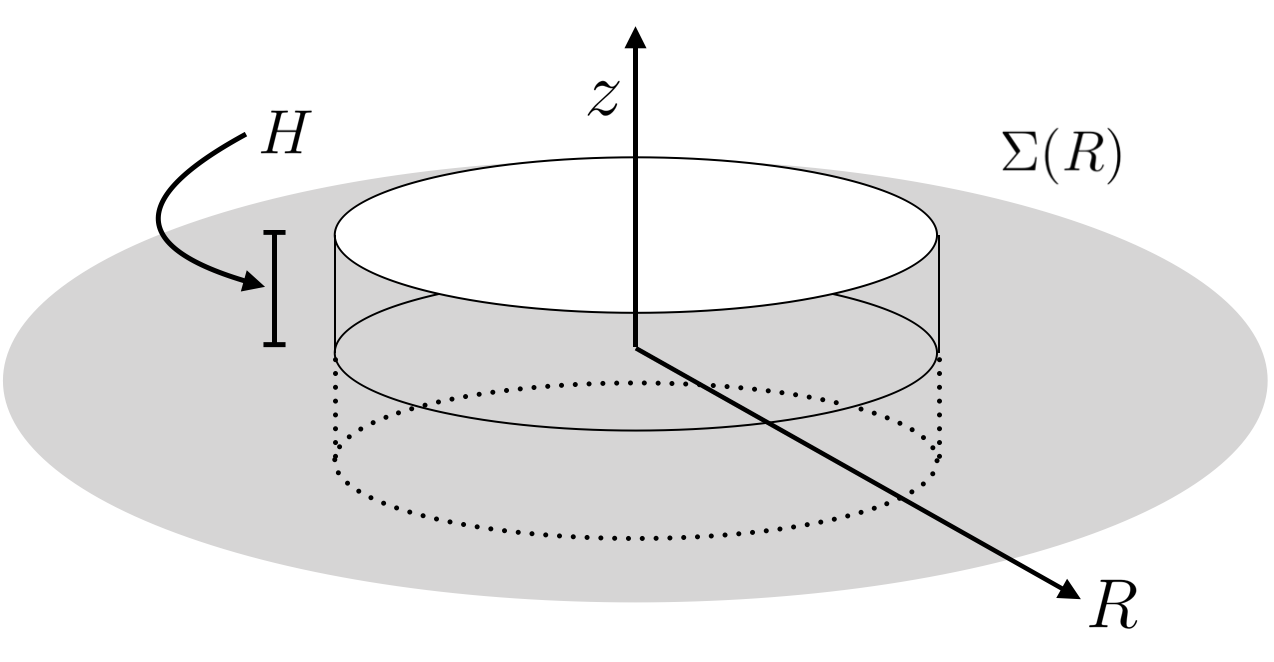
\includegraphics[width=0.8\columnwidth]{Anexos/disk_surface.png}
\caption{Superficie gaussiana cerca al plano ecuatorial para el disco delgado }
\label{fig:disk_surface}
\end{figure}


\begin{eqnarray}
 4\pi G \Sigma(R) A &=& \left (  \left [ \frac{\partial \Phi}{ \partial z }   \right ]_{z=0+} - \left [ \frac{\partial \Phi}{ \partial z }   \right ]_{z=0-} \right ) \times A,  \\
 4\pi G \Sigma(R) &=& \left (  \left [ \frac{\partial \Phi}{ \partial z }   \right ]_{z=0+} - \left [ \frac{\partial \Phi}{ \partial z }   \right ]_{z=0-} \right ) \times, \\
    &=& -\int_0^{\infty} k f(k) e^{-k0+}J_0(kR) dk - \int_0^{\infty} kf(k) e^{-k0-} J_0(kR) dk, \\
    &=& -\int_0^{\infty} k f(k) J_0(kR) dk - \int_0^{\infty} kf(k)  J_0(kR) dk, \\
    &=& -2\int_0^{\infty} k f(k) J_0(kR) dk, \\
 \end{eqnarray}

por lo tanto la densidad superficial de masa es

$$ \Sigma(R) = -\frac{1}{2\pi G} \int_0^{\infty} k f(k) J_0(kR) dk $$
 
 y por la transformada de Hankel, ecuación (\ref{Hankel}),
 
 $$ f(k) = -2\pi G \int_0^{\infty} \Sigma(R) J_0(kR)R dR. $$

 Entonces, una vez conocida la distribución superficial de masa $\Sigma(R)$, se puede conocer la función de peso $f(k)$ y luego por la ecuación
 
\begin{equation}
    \Phi(R,z) = \int_0^{\infty} \Phi_k(R,z) f(k) dk
\end{equation}
  
  se obtiene el potencial $\Phi$.
 

\chapter{Anexo: Ecuaciones de Jeans en sistemas esféricos}

Partiendo de las coordenadas esféricas polares y momentos canónicamente conjugados:

\begin{align*}
\textbf{q} &= (r, \theta, \phi) \\
\textbf{p} &= (p_r, p_\theta, p_\phi) \\
p_r &= v_r,  & d p_r &= d v_r \\
p_\theta &= r v_\theta,  & d p_\theta &= r d v_\theta \\
p_\phi &= r sin \theta v_\phi,  & d p_\phi &= r sin \theta d v_\phi \\
\int d^3 p f &= \int d p_r d p_\theta d p_\phi f = r^2 sin \theta \int d^3 v  f = r^2 sin \theta \nu \\
\frac{\partial }{ \partial p_r} (p_r f) &= f + p_r \frac{\partial f}{\partial p_r} \\
\frac{\partial }{\partial p_r} (p_r f) - f &= p_r \frac{\partial f}{\partial p_r}
\end{align*}


con el Hamiltoniano (\ref{Hamiltonian_potential}):

\begin{equation}
H = \frac{1}{2} \left [ p_r^2 + \left ( \frac{1}{r} p_\theta  \right )^2 + \left ( \frac{1}{r sin \theta} p_\phi  \right )^2 \right ] + \Psi (r),
\end{equation}

la ecuación de Boltzmann en coordenadas generalizadas (\ref{Boltzmann_eq_gener}) es:

\begin{equation}
p_r \frac{\partial f}{\partial r} + \frac{p_\theta}{r^2} \frac{\partial f}{\partial \theta} - \left ( \frac{d \Psi}{d r}  - \frac{p_\theta^2}{r^3} - \frac{p_\phi^2}{r^3 sin^2\theta} \right ) \frac{\partial f}{\partial p_r} + \frac{p_\phi^2 cos \theta}{r^2 sin^3\theta} \frac{\partial f}{\partial p_\theta} = 0
\end{equation}

donde se ha asumido que el sistema es esférico e independiente del tiempo. Luego, multiplicando por $p_r$ e integrando en todos los momentos canónicamente conjugados, se tiene que cada término de la integral es:

\begin{align}
\int p_r^2 d^3 p \frac{\partial f}{\partial r} &= \frac{\partial }{\partial r} \int p_r^2 d^3 p f = \frac{\partial }{\partial r} (r^2 sin \theta \nu \overline{p_r^2}) \\
\int p_r \frac{p_\theta}{r^2} d^3 p \frac{\partial f}{\partial \theta} &= \int v_r r v_\theta \frac{1}{r^2} r^2 d^3 v \frac{\partial }{\partial \theta} = r sin \theta \frac{\partial }{\partial \theta} \int v_r v_\theta d^3v f \\
& = r sin \theta \frac{\partial }{\partial \theta} (\overline{v_r v_\theta } \nu) = sin \theta \frac{\partial }{\partial \theta} (\overline{p_r p_\theta } \nu) \\
\int d^3 p \left ( \frac{d \Psi}{d r}  - \frac{p_\theta^2}{r^3} - \frac{p_\phi^2}{r^3 sin^2\theta} \right ) p_r \frac{\partial f}{\partial p_r} & = \int  d^3 p \left ( \frac{d \Psi}{d r} - \frac{p_\theta^2}{r^3} - \frac{p_\phi^2}{r^3 sin^2\theta} \right ) \left [ \frac{\partial }{\partial p_r} (p_r f) - f \right ] \\
\label{Boltzmann_third_int}
& = \int  d^3 p \left ( \frac{d \Psi}{d r} - \frac{p_\theta^2}{r^3} - \frac{p_\phi^2}{r^3 sin^2\theta} \right ) \frac{\partial }{\partial p_r} (p_r f)\\
&- \int  d^3 p \left ( \frac{d \Psi}{d r} - \frac{p_\theta^2}{r^3} - \frac{p_\phi^2}{r^3 sin^2\theta} \right ) f \\
& = \nu r^2 sin \theta \left ( \frac{d \Psi}{d r} - \frac{ \overline{p_\theta^2} }{r^3} - \frac{ \overline{p_\phi^2} }{r^3 sin^2\theta} \right )
\end{align}

donde, por el teorema de la divergencia (\ref{Div_teorem}) se tiene que la función de distribución en (\ref{Boltzmann_third_int}) se anula en la superficie $S$ donde las velocidades son muy grandes. De esta forma:

\begin{equation}
\frac{\partial }{\partial r} (r^2 sin \theta \nu \overline{p_r^2}) + sin \theta \frac{\partial }{\partial \theta} (\overline{p_r p_\theta } \nu) + \nu r^2 sin \theta \left ( \frac{d \Psi}{d r} - \frac{ \overline{p_\theta^2} }{r^3} - \frac{ \overline{p_\phi^2} }{r^3 sin^2\theta} \right ) = 0.
\end{equation}

y por la misma razón que la velocidad media en (\ref{Mean_vel}) se anula, el término $\overline{v_r v_\theta}$ se anula. Dividiendo entre $r^2 sin \theta$ y volviendo a las velocidades se obtiene que:

\begin{align}
\frac{d (\nu \overline{v_r^2})}{dr} + \nu \left ( \frac{d \Psi}{d r} + \frac{2 \overline{v_r^2}-\overline{v_\theta^2}-\overline{v_\phi^2}}{r} \right ) & = 0 \\
\frac{d (\nu \overline{v_r^2})}{dr}  + 2 \frac{\beta}{r} \nu \overline{v_r^2} & = - \nu \frac{d \Psi}{d r}
\end{align}

que corresponde a la ecuación de Jeans radial.



\chapter{Anexo: Nombrar el anexo C de acuerdo con su contenido}
MANEJO DE LA BIBLIOGRAF\'{I}A: la bibliograf\'{\i}a es la relaci\'{o}n de las fuentes documentales consultadas por el investigador para sustentar sus trabajos. Su inclusi\'{o}n es obligatoria en todo trabajo de investigaci\'{o}n. Cada referencia bibliogr\'{a}fica se inicia contra el margen izquierdo.\\

La NTC 5613 establece los requisitos para la presentaci\'{o}n de referencias bibliogr\'{a}ficas citas y notas de pie de p\'{a}gina. Sin embargo, se tiene la libertad de usar cualquier norma bibliogr\'{a}fica de acuerdo con lo acostumbrado por cada disciplina del conocimiento. En esta medida es necesario que la norma seleccionada se aplique con rigurosidad.\\

Es necesario tener en cuenta que la norma ISO 690:1987 (en Espa\~{n}a, UNE 50-104-94) es el marco internacional que da las pautas m\'{\i}nimas para las citas bibliogr\'{a}ficas de documentos impresos y publicados. A continuaci\'{o}n se lista algunas instituciones que brindan par\'{a}metros para el manejo de las referencias bibliogr\'{a}ficas:\\

\begin{center}
\centering%
\begin{tabular}{|p {7.5 cm}|p {7.5 cm}|}\hline
\arr{Instituci\'{o}n}&Disciplina de aplicaci\'{o}n\\\hline%
Modern Language Association (MLA)&Literatura, artes y humanidades\\\hline%
American Psychological Association (APA)&Ambito de la salud (psicolog\'{\i}a, medicina) y en general en todas las ciencias sociales\\\hline
Universidad de Chicago/Turabian &Periodismo, historia y humanidades.\\\hline
AMA (Asociaci\'{o}n M\'{e}dica de los Estados Unidos)&Ambito de la salud (psicolog\'{\i}a, medicina)\\\hline
Vancouver &Todas las disciplinas\\\hline
Council of Science Editors (CSE)&En la actualidad abarca diversas ciencias\\\hline
National Library of Medicine (NLM) (Biblioteca Nacional de Medicina)&En el \'{a}mbito m\'{e}dico y, por extensi\'{o}n, en ciencias.\\\hline
Harvard System of Referencing Guide &Todas las disciplinas\\\hline
JabRef y KBibTeX &Todas las disciplinas\\\hline
\end{tabular}
\end{center}

Para incluir las referencias dentro del texto y realizar lista de la bibliograf\'{\i}a en la respectiva secci\'{o}n, puede utilizar las herramientas que Latex suministra o, revisar el instructivo desarrollado por el Sistema de Bibliotecas de la Universidad Nacional de Colombia\footnote{Ver: www.sinab.unal.edu.co}, disponible en la secci\'{o}n "Servicios", opci\'{o}n "Tr\'{a}mites" y enlace "Entrega de tesis".

\end{appendix}